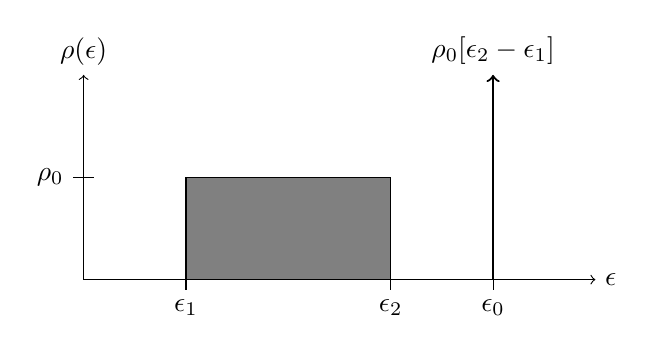
\begin{tikzpicture}[
        scale=1.3,
    ]
    \draw[->] (0, 0) -- (5, 0) node[right] {$\epsilon$};
    \draw[->] (0, 0) -- (0, 2) node[above] {$\rho(\epsilon)$};

    \draw[draw, fill=gray] (1, 0) rectangle +(2, 1);

    \draw[thick, ->] (4, 0) -- ++(0, 2) node[above] {$\rho_0 [\epsilon_2 - \epsilon_1]$};

    \draw (1, .1) -- ++(0, -0.2) node[below] {$\epsilon_1$};
    \draw (3, .1) -- ++(0, -0.2) node[below] {$\epsilon_2$};
    \draw (4, .1) -- ++(0, -0.2) node[below] {$\epsilon_0$};

    \draw (.1, 1) -- ++(-0.2, 0) node[left] {$\rho_0$};
\end{tikzpicture}
